\documentclass{anstrans}
%\documentclass[times, 10pt]{article}

\usepackage{graphicx} % allows inclusion of graphics
\usepackage{booktabs} % nice rules (thick lines) for tables
% \usepackage{microtype} % improves typography for PDF
% \usepackage{xcolor}
\usepackage{amsmath}
\usepackage{tabulary}
\usepackage{bm}
\usepackage{tikz}
% \usepackage{verbatim}
\usetikzlibrary{arrows,shapes}
\usepackage{subfigure}
% \usepackage{braket}
\usepackage{amssymb}
\usepackage{url}
\usepackage[figuresright]{rotating}


% put your own definitions here:
\newcommand{\SN}{S$_N$}
\renewcommand{\vec}[1]{\bm{#1}} %vector is bold italic
\newcommand{\vd}{\bm{\cdot}} % slightly bold vector dot
\newcommand{\grad}{\vec{\nabla}} % gradient
\newcommand{\ud}{\mathop{}\!\mathrm{d}} % upright derivative symbol
%   \newcommand{\cZ}{\cal{Z}}
%   \newtheorem{def}{Definition}[section]
%   ...
\newcommand{\oper}[1]{\mathcal{#1}}
\newcommand{\EQ}[1]{Eq.~(\ref{#1})}               %-- Eq. (refeq)
\newcommand{\EQUATION}[1]{Equation~(\ref{#1})}    %-- Equation (refeq)
\newcommand{\FIG}[1]{Fig.~\ref{#1}}               %-- Fig. refig
\newcommand{\FIGURE}[1]{\FIG{#1}}          %-- Figure refig
\newcommand{\TAB}[1]{Table~\ref{#1}}              %-- Table tablref
\newcommand{\EQS}[2]{Eqs.~(\ref{#1})--(\ref{#2})}      
\newcommand{\EQUATIONS}[2]{Equations~(\ref{#1})--(\ref{#2})}       
\newcommand{\EQSTWO}[2]{Eqs.~(\ref{#1})~and~(\ref{#2})}         
\newcommand{\EQUATIONSTWO}[2]{Equations~(\ref{#1})~and~(\ref{#2})}           
\newcommand{\BOXEQ}[1]{\mbox{\fboxsep=.13in $$
        \framebox{$ #1 $} $$ } }    %-- box around equation
\newcommand{\SEC}[1]{Section~\ref{#1}}               %-- Eq. (refeq)
\newcommand{\REF}[1]{Ref.~\citen{#1}}               %-- Eq. (refeq)
\DeclareMathOperator*{\dotp}{{\scriptscriptstyle \stackrel{\bullet}{{}}}}


% add words to TeX's hyphenation exception list
%\hyphenation{author another created financial paper re-commend-ed Post-Script}

% declarations for front matter

\title{Updating a PWR Simulator in Python}
\author{Richard L. Reed, Jacob W. Hayhurst, Shravan D. Gangadhara, Jeremy A. Roberts}

\institute{
    Mechanical and Nuclear Engineering, Kansas State University, Manhattan, KS
}

\email{rlreed@k-state.edu, hayhujac@k-state.edu, shravandg@k-state.edu, jaroberts@k-state.edu}

\begin{document}
    
    \section{Introduction}
    
    A nuclear reactor is a complicated system that is comprised of many systems  
    and components.  In order to fully model a reactor, several 
    approximations and correlations must be used for a 
    real-time simulation.  In 1984 as part of a doctoral dissertation at 
    Massachusetts Institute of Technology (MIT), a 
    FORTRAN 77 program 
    was developed to simulate a four-loop, Westinghouse pressurized water reactor 
    (PWR) \cite{kao1984}.  The program was later called PRISM and extended to include
    a comprehensive set of features accessible in a DOS-based user interface.  
    This present work seeks to update the original PRISM program
    for cross platform deployment using the Python language.
    
    \subsection{Motivation}
    
    A need was identified in the 1980s for a better-than-real-time simulation of a nuclear 
    reactor.  Ideally, such a simulation would incorporate all 
    reactor systems including both primary and secondary sides as well as the 
    ability to run within tripped or startup conditions.  PRISM was created to fill that 
    need, and was developed in the FORTRAN 77 programming language.  However, the user
    interface of PRISM uses packages that are no longer widely available.
    In fact, the current procedure for running PRISM requires using an emulator for the DOS 
    operating system. Such requirements make use of PRISM in the average class somewhat
    tedious.
    
    \subsection{Project Goals}
    
    This work has been focused on updating PRISM into the Python programming 
    language, which can run on all modern operating systems and will continue to do 
    so for the foreseeable future.  The effort is divided into two teams, 
    which focus on the back-end physics models and the graphical user interface (GUI)
    respectively.  
    
    The physics team is currently reverse engineering the models used for the original 
    PRISM implementation and will then update the models as needed.  Due to the advancement
    in computing technology since the original design, the physics models may be made more
    robust while maintaining the real-time modeling capabilities.  Additionally,
    the new implementation will be fully object oriented, which will allow smooth
    design and incorporation of future improvements or additions to the simulator.
    
    It is important that the new implementation uses regression testing based on
    output from the original
    PRISM design to leverage the significant validation previously done for  
    PRISM.  Upon completion, the new implementation will have the capability to 
    show the operating conditions (i.e., temperature, pressure, trip status, etc.) 
    within each of the major components within the reactor.  With the ability to control
    various systems, e.g., the control rod positions, the user will be able to simulate
    the real time dynamics of the nuclear reactor, which would be instrumental for 
    operators or students in an educational setting.
    
    To this end, the GUI team is focused on developing an interface that is portable
    to many devices and operating systems including Windows, iOS, Linux, and mobile 
    platforms.  The Kivy Python library \cite{kivy} was chosen to create the GUI for its 
    clean design and cross-platform capabilities.  In other words, the same Kivy
    code can be used to generate mobile applications for Android and iOS devices.
    The primary goal for the GUI is to reproduce the original user interface using Kivy
    and then to modernize the GUI as well as improve the data availability for the user.
    
    \section{Original PRISM}
    
    In the original simulator \cite{kao1984}, only the primary systems were 
    included in the simulation.  Additional work was completed 
    to add models for secondary systems including steam generators as well as 
    various alarms.  The additional work led to the completion
    of the original PRISM which 
    was a fully-featured, complete reactor systems model. However, documentation
    of the models for the secondary systems is not available as part of the original
    project.  Hence, the physics
    team had to recreate the models from the original source code in order to revise
    and update the capabilities. A summary of these models is available elsewhere
    \cite{github-io}
    
    \begin{figure*}[t!]
        \centering
        \begin{subfigure}[Landing page for the new implementation]{
            \centering
            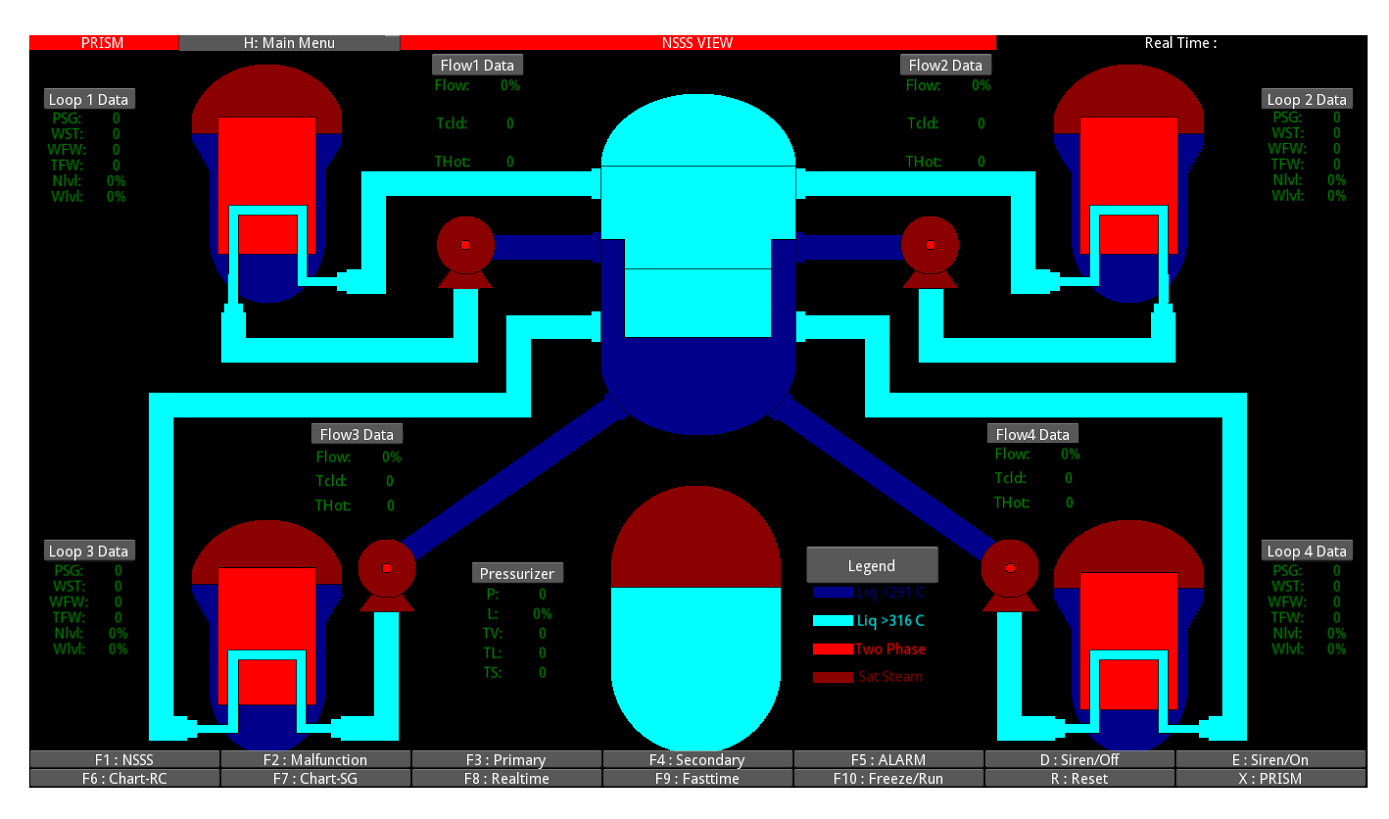
\includegraphics[width=1.8\columnwidth]{newPrism}
            \label{fig:new}}
        \end{subfigure}
        
        \begin{subfigure}[Landing page for original PRISM]{
            \centering
            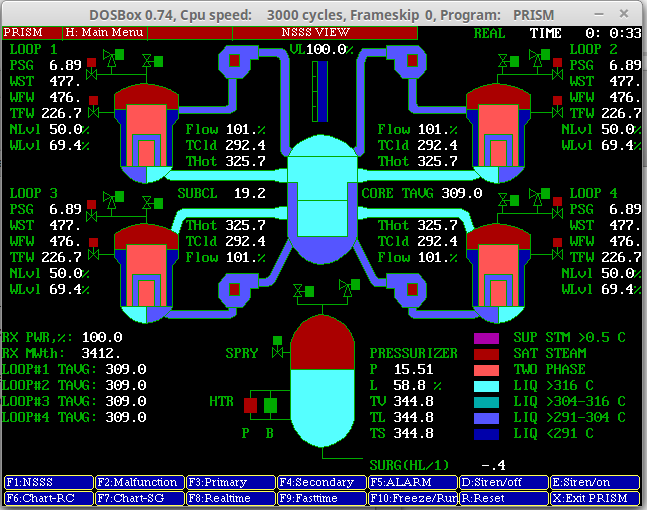
\includegraphics[width=1.5\columnwidth]{prism}
            \label{fig:old}}
        \end{subfigure}\hfill
        \caption{Comparison between the present work and the original implementation}
    \end{figure*}
    
    \section{Python Implementation - Physics}
    The current work divided the reactor into three major systems, which included
    the pressurizer, reactor vessel, and loops.  Each system can incorporate several
    components, e.g., the loop contains the steam generator, cold leg, pump, etc.,
    which allows each system to be developed independently and linked via inlet
    and outlet boundary conditions on the coolant flow.  Each of these components
    are modeled as independent classes, which greatly simplifies the 
    addition of new components within a system or additional systems 
    entirely, e.g., a thermal storage system.
    
    The most robust model is the reactor vessel, which is based on a 
    point kinetics model with six delayed groups that is linked with a 
    lumped-fuel model to handle heat transfer to the bulk coolant from the fuel rods.
    Additional correlations
    are used to approximate heat transfer coefficients and other resistances to 
    heat flow.  Control rod positions as well as reactor poison concentrations are
    tracked during the simulation to determine the amount of excess reactivity in the core,
    which correlates with the power in the reactor vessel.  Furthermore, the model was adapted to allow for operation outside of normal 
    conditions, e.g., startup conditions, two phase flow in the vessel, reverse flow.
    
    Many of the components outside the reactor vessel, e.g., within the loop, are
    based on a combined mass and energy balance coupled with a momentum balance. Again,
    these equations are augmented for non-standard flow conditions such as reverse
    flow or pipe breakages.
    
    \section{Python Implementation - GUI}
    To redesign the GUI, the first project was to develop a system of mini applications
    in Kivy, and the final GUI would be build upon these building block.  Thus far,
    the suite of mini apps is nearly complete and 
    includes components including sliders, buttons, basic shapes, dropdown menus, 
    and more. The suite is available via a git repository \cite{kivyapps}. 
    
    Kivy itself is a relatively new library for Python and does not yet have
    an extensive documentation for its capabilities as compared to popular 
    Python libraries, e.g., Numpy.  The mini apps developed for the current 
    project may serve to extend the Kivy documentation as well as their set of examples.
    
    The next step is to reproduce the original PRISM GUI in Kivy.  A first pass has
    been completed, shown in \FIG{fig:new}.  For comparison, the original 
    GUI is shown in \FIG{fig:old}.  These figures show the landing page for the program.
    In addition to the first page are several pages of sliders, plots, and data
    presentation that are not shown in this summary.
    
    Considerable updates to the GUI are planned, which will update the design to
    a modern approach.  The currently presented graphics are merely a proof of
    concept using Kivy to reproduce the existing design.  
    
    
    \section{Conclusions}
    
    The goal of this present work is to update and improve a teaching tool for 
    both students and reactor operators.  Originally, PRISM was created as part
    of a PhD project in FORTRAN 77, but the code no longer works readily on modern 
    operating systems.  Python was chosen to rewrite the program
    because of the ease of use of the Python modules including Kivy as well as
    the portability of the program to various operating systems.
    
    This project aims to develop desktop and mobile versions of the software, 
    allowing the user flexibility in choice of platform.  This simulator is scheduled
    to be deployed in time for a live demonstration at the 2016 Annual ANS meeting.  
    
    The project aims to produce a reactor simulator that will showcase the dynamics
    of a PWR system in real-time under various conditions.  Some potential scenarios
    include startup conditions, scram operations, or failure conditions such as
    a break in a coolant leg.  
    
    The user will be able to induce various failure scenarios and the program will
    simulate how the reactor will behave.  The simulation will include a suite of 
    monitoring functions that will allow automatic systems to attempt to adapt to
    the changing conditions, e.g., control rod movement.  This program will provide
    an educational resource for anyone learning about nuclear reactor kinetics or
    dynamics of a reactor system.
    
    \section{Acknowledgements}
    
    This work is supported in part by the Kansas State Electrical Power Affiliates
    Program (EPAP).
    
\bibliographystyle{ans}
\bibliography{bibliography}
    
\end{document}
